\scanpage{136}
% archive sheet number: 135
\figure{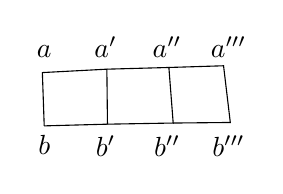
\begin{tikzpicture}[x=.78cm,y=.72cm]
\draw (0,0)--(-.03,.94)--(1.02,1)--(1.03,.03)--(0,0);
\draw (1.02,1)--(2.03,1.03)--(2.10,.05)--(1.03,.03);
\draw (2.03,1.03)--(2.92,1.06)--(3.03,.06)--(2.10,.05);
\foreach \x/\t/\b in {0/a/b,1/{a'}/{b'},2/{a''}/{b''},3/{a'''}/{b'''}}{
\node[above] at (\x,1.03){$\t$};\node[below] at (\x,0){$\b$};}
\end{tikzpicture}}
n'existe pas dans graphe cubique, car on trouve que les \deleted{triangles de bases}\inserted{$3^{\mathrm e}$ sommet} des triangles de bases $(a''',b''')$ égale celui du triangle de bases $(a^{\deleted{\unsure{''}}},b^{\deleted{\unsure{'|''}}})$ et $(a^{\deleted{\unsure{''|'}}},b')$, ce qui sont donc égaux -- absurde d'après étude du carré

Conséquence : pas de prismes à bases pentagonale et hexagonale. Par contre $\unsure{\exists|\nexists}$ prismes à base carré, i.e. cubes.

\margin{\uline{NB} : Carré définit pt, \unsure{paire de tripaires|paire de triplets|paire de tripodes}, une bibase, un triangle\ldots}

Carrés de centre un pt donné $a$ : d'abord la \deleted{\unsure{cat.}}donnée des graphes cubiques à pt marqué $a$, équivaut à celle d'un ens $I$ de card. $5$ et d'un torseur $T$ sous $V_I=(\mathbb F_2^I)'$ \inserted{(de dim $4$ sur $\mathbb F_2$)} engendré par des $e_i$ $(i\in I)$ avec la seule relation $\sum e_i=0$. L'ens des pts non liés à $a$ est $T$. Les \deleted{\unsure{de|donnée}} carrés sont les sous-espaces affines de dim $2$, dont l'espace des translations soit engendrés par $2$ parmi les $e_i$, \deleted{\unsure{donc}}\inserted{corr.} à une partie $I'$ de $I$ de cardinal $2$. Si $V_{(I')}$ est le sous-vectoriel correspondant, les carrés en question correspondent aux pts de $T/V_{(I')}$, ou aux restrictions du groupe structural de $V_I$ à $V_{(I')}\simeq\mathbb F_2^{I'}$. $[$Donc la cat. des graphes cubiques $+$ carrés équivaut à celle des \deleted{couples}\inserted{triplets} \deleted{$(\unsure{I'},\unsure{T'})$} $(\unsure{I'|I''}$ ens. de card. $2$, $T'$ torseur sous $\mathbb F_2^{I'}$, $I''(=I\backslash I')$ ens de card. $3)$ i.e. $(\mathrm{Ens})_{2,2}\times\mathrm{Ens}_3\simeq\text{Carré}\times(\mathrm{Ens})_3$
